\documentclass[a4paper,norsk,12pt,oneside]{article}
% To use norwegian
\usepackage[utf8]{inputenc}
\usepackage[T1]{fontenc}
\usepackage[norsk]{babel}
% math
\usepackage{amsmath}
\usepackage{amsfonts}
\usepackage{amssymb}

\usepackage{graphicx} % images
\usepackage{float}
\usepackage{enumerate}
\usepackage{fancyvrb} % code
\usepackage{algorithm2e} % algorithm
% For listing
\usepackage{listings} % code with color
\usepackage{courier}
\usepackage{caption}
\usepackage{color}

\title{CompPhys, project 1}
\author{Idun Kløvstad}
\date{\today}  

% Command for L'Hopital's rule (requires extarrows-package)
\newcommand{\Heq}[1]{\xlongequal[\mathrm{L'H}]{\left[#1\right]}}

% Double underline
\newcommand{\dul}[1]{\underline{\underline{#1}}}

% Custom operators
\DeclareMathOperator{\nul}{Nul\,}
\DeclareMathOperator{\Proj}{Proj\,}
\DeclareMathOperator{\Sp}{Sp\,}
\DeclareMathOperator{\res}{Res\,}
\DeclareMathOperator{\Log}{Log\,}

% Allow displayed page breaks
\allowdisplaybreaks

% Settings for listings
\definecolor{dkgreen}{rgb}{0,0.6,0}
\definecolor{gray}{rgb}{0.5,0.5,0.5}
\definecolor{mauve}{rgb}{0.58,0,0.82}

\lstset{%
  %language=python,                     % the language of the code
  basicstyle=\footnotesize\ttfamily,   % the size of the fonts that are used for the code
  numbers=left,                        % where to put the line-numbers
  numberstyle=\tiny,                   % the style that is used for the line-numbers
  stepnumber=2,                        % the step between two line-numbers. If it's 1, each line will be numbered
  numbersep=5pt,                       % how far the line-numbers are from the code
  extendedchars=true,
  %backgroundcolor=\color{white},       % choose the background color. You must add \usepackage{color}
  %showspaces=false,                    % show spaces adding particular underscores
  showstringspaces=false,              % underline spaces within strings
  %showtabs=false,                      % show tabs within strings adding particular underscores
  %frame=single,                        % adds a frame around the code
  frame=b,                             % adds a line at the bottom
  %rulecolor=\color{black},             % if not set, the frame-color may be changed on line-breaks within not-black text (e.g. commens (green here))
  tabsize=2,                           % sets default tabsize to 2 spaces
  %captionpos=b,                        % sets the caption-position to bottom
  breaklines=true,                     % sets automatic line breaking
  breakatwhitespace=false,             % sets if automatic breaks should only happen at whitespace
  %title=\lstname,                      % show the filename of files included with \lstinputlisting; also try caption instead of title
  keywordstyle=\color{blue},           % keyword style
  commentstyle=\color{dkgreen}\textit, % comment style
  stringstyle=\color{mauve},           % string literal style
  %escapeinside={\%*}{*)},              % if you want to add LaTeX within your code
  %morekeywords={*,...},                % if you want to add more keywords to the set
  xleftmargin=-20pt,
  xrightmargin=-20pt,
  framexleftmargin=19pt,
  framexbottommargin=4pt,
  framexrightmargin=21pt,
} 

% caption for listing
\newlength{\mycapwidth}\setlength{\mycapwidth}{\textwidth}
\addtolength{\mycapwidth}{75pt}
\DeclareCaptionFont{white}{\color{white}}
\DeclareCaptionFormat{listing}{\colorbox[cmyk]{0, 0, 0, 0.8}
    {\parbox{\mycapwidth}{\hspace{15pt}#1#2#3}}}
\captionsetup[lstlisting]{format=listing,labelfont=white,textfont=white, 
    singlelinecheck=false, margin=-40pt, font={bf,footnotesize}}


\begin{document}
\maketitle
\newpage 

\begin{abstract}
    This project will be looking at how to solve the one-dimensional Poisson equation with
Dirichlet boundary conditions by rewriting it as a set of linear equations. The numerical 
calculations will be done with three different methods, and these methods will be compared 
to each other. The relative error of the numerical solution will also be taken into
consideration. 
\end{abstract}

Full program and additional files can be found here:

https://github.com/idunklo/CompPhys\_project1

\section{Introduction}

The purpose of this project is to solve the one-dimensional Poisson equation with
Dirichlet boundary conditions by rewriting it as a set of linear equations. 

The equation we want to solve then looks like this:
\begin{equation}\label{eq:1}
    -u''(x) = f(x), \ x \epsilon (0,1), \ u(0) = u(1) = 0.
\end{equation}

We will look at three different methods for calculating a numerical solution for this problem and the 
numerical solution will then be compared with a known closed-form solution to find
the relative error for a different number of grid-points.  

As the calculation to find this numerical solution is done
in three different ways, it is also relevant to look at the difference between them.
In this project we will compare how general the method is to the
number of floating point operations and the CPU time.
%TODO rewrite this section so it is readable 

\section{Theory}

As stated in the introduction, the equation we will solve in this 
project is equation ~\ref{eq:1}. 

To do this, we start by defining the discretizes approxiamtion as \(v_i\), with grid points 
\(x_i = ih\). The interval we are looking at is from \(x_0 = 0\) to \(x_{n+1} = 1\). 
The step length, h, is defined as \(h = \frac{1}{n+1}\). From equation ~\ref{eq:1}
we have the boundary conditions \(v_0 = v_{n+1} = 0\). 
With this information we can approximate the second derivative of u with

\begin{equation}\label{eq:2}
    -\frac{v_{i+1} + v_{i-1} - 2v_i}{h^2} = g_i \ for \ i = 1, \cdots, n
\end{equation}

where \(g_i\) is given as \(g(x_i)\).

If we rewrite equation ~\ref{eq:2} by multiplying with \(h^2\) on both sides
and write it out with different values for i like this

\begin{align*}
    -v_2 + 2v_1 - v_0 &= h^2g_1\\
    -v_3 + 2v_2 - v_1 &= h^2g_2\\
    -v_4 + 2v_3 - v_2 &= h^2g_3\\
    &\vdots \\
    -v_{n+1} + 2v_n - v_{n_1} &= h^2g_{n}
\end{align*}, 

we can notice a pattern. As the boundary conditions are set to \(v_0 = v_{n+1} = 0\), we see that
equation ~\ref{eq:2} can be written as a linear set of equations on the form

\begin{equation*}
    \textbf{A} \textbf{v} = \textbf{f}
\end{equation*} 

Where \(\textbf{A}\) is an \(n \ x \ n\) tridiagonal matrix with \(-1\) on the lower and 
upper diagonal and \(2\) on the main diagonal and \(f_i = h^2 g_i\). The linear set will
then look like this:

\begin{align}
	\label{matrix_A}	
	\begin{bmatrix}
		2 & -1 & 0 & \hdots & \hdots & \hdots \\
		-1 & 2 & -1 & 0 & \hdots & \hdots \\
		& -1 & 2 & -1 & \hdots & \hdots \\
		& \hdots & \hdots & \hdots & \hdots & \hdots \\ 
		&& \hdots & -1 & 2 & -1 \\
		&& \hdots & \hdots & -1 & 2 
	\end{bmatrix} \begin{bmatrix}
	v_1 \\ v_2 \\ v_3 \\ \hdots \\ v_{n-1} \\ v_n
	\end{bmatrix} &= \begin{bmatrix}
	f_1 \\ f_2 \\ f_3 \\ \hdots \\ f_{n-1} \\ f_n
	\end{bmatrix}
\end{align}.  

This can be verified by doing the matrix vector multiplication.

If we assume that the source term is \(g(x) = 100e^{-10x}\) and keep the
same interval and boundary conditions, the differential equation has a 
closed-form solution given by.
\begin{equation*}
    u(x) = 1-(1-e^{-10})x - e^{-10x}
\end{equation*} 

When calculating a solution for the equation numerically, this analytical
solution can be used in comparison with our numerical one. If we compare 
for different number of grid points, \(n\), it is expected that the numerical solution
will get closer to the analytical one with a higher number of grid points. 

For a more general expression, we can rewrite the
tridiagonal matrix \(\textbf{A}\) in terms of vectors
\(a, b, c\) of length \(1 : n\). That gives us the following linear equation:

\begin{align}\label{eq:general}
	\label{full eq Ax=f}	
	\begin{bmatrix}
		b_{1} & c_{1} & 0 & \hdots & \hdots & \hdots \\
		a_{2} & b_{2} & c_{2} & 0 & \hdots & \hdots \\
		& a_{3} & b_{3} & c_{3} & \hdots & \hdots \\
		& \hdots & \hdots & \hdots & \hdots & \hdots \\ 
		&& \hdots & a_{n-1} & b_{n-1} & c_{n-1} \\
		&& \hdots & \hdots &  & b_{n} 
	\end{bmatrix} \begin{bmatrix}
	v_1 \\ v_2 \\ v_3 \\ \hdots \\ v_{n-1} \\ v_n
	\end{bmatrix} &= \begin{bmatrix}
	f_1 \\ f_2 \\ f_3 \\ \hdots \\ f_{n-1} \\ f_n
	\end{bmatrix}
\end{align}. 

The endpoints are not included as we have boundary conditions that result in a fixed 
value for \(v_i\). 

When solving the equation numerically, we will get a relative error.
To compute this relative error we set up 

\begin{equation*}
    \epsilon_i = log_{10} \left ( \left | \frac{v_i - u_i}{u_i} \right | \right )
\end{equation*}, 
as a function of \(log_{10}(h)\), where\(v_i\) is the numerically calculated solution
in each timestep and \(u_i\) is the closed-form solution in each timestep. The maximum of
the relative error for each \(n\) will be the relative error used. 
As when we plot the numerical solution against the analytical one, we expect the relative 
error to be smaller as we increase the number of grid points. But as we are calculating 
on a computer, we have to consider that at some point when the numbers get high,
we will try to subtract to very similar numbers from each other and we can expect that the relative
error will start to increase again. 

\section{Algorithms and implementations}

There are several different ways to solve this numerically. We will look at three methods.
Using the different methods should give the same output, down to numerically precition, 
but is more and less generalized and therefore have a different number of floating point
operations which will have an impact on the CPU-time. 

\subsection{General algorithm for a tridiagonal matrix}\label{subsec:general}

First we look at the tridiagonal matrix \(\textbf{A}\) assuming different values
for the matrix elements. 
We are then looking at the linear set ~\ref{eq:general}. 

To find a general algorithm for this problem, we start by eliminating the lower diagonal.
This is done by doing the following to each row: 

\begin{equation}\label{eq:rowred}
    row_n - row_{n-1} \frac{a_n}{b_{n-1}}
\end{equation}

This eliminates the a-vector, leaves the c-vector unchanged and updates the b-vector as follows:


\begin{align*}
    \tilde{b_2} &= b_2 - c_1 \frac{a_2}{\tilde{b_1}}\\\\
    \tilde{b_3} &= b_3 - c_2 \frac{a_3}{\tilde{b_2}}\\\\
    \tilde{b_4} &= b_4 - c_3 \frac{a_4}{\tilde{b_3}}\\
    &\vdots \\
    \tilde{b_n} &= b_n - c_{n-1} \frac{a_n}{\tilde{b_{n-1}}} 
\end{align*}. 

It is important to remember that when we change the left side of the equation, the right side
must also be updated in the same way, which gives 

\begin{align*}
    \tilde{f_2} &= f_2 - f_1 \frac{a_2}{\tilde{b_1}}\\\\
    \tilde{f_3} &= f_3 - f_2 \frac{a_3}{\tilde{b_2}}\\\\
    \tilde{f_4} &= f_4 - f_3 \frac{a_4}{\tilde{b_3}}\\
    &\vdots \\
    \tilde{f_n} &= f_n - f_{n-1} \frac{a_n}{\tilde{b_{n-1}}} 
\end{align*}.

Summarized, this can be written as an algorithm called forward substitution,
which I have implemented in my program in the following way:

\lstinputlisting[language=C++, title = Forward substitution, firstline=49, lastline=55]{project1.cpp}

By doing the foreward substitution, we are left with this new updated linear set

\begin{align}\label{eq:general}
	\label{full eq Ax=f}	
	\begin{bmatrix}
        b_{1} & c_{1} & 0 & \hdots & \hdots & \hdots \\
        0 & \tilde{b_{2}} & c_{2} & 0 & \hdots & \hdots \\
        & 0 & \tilde{b_{3}} & c_{3} & \hdots & \hdots \\
		& \hdots & \hdots & \hdots & \hdots & \hdots \\ 
        && \hdots & 0 & \tilde{b_{n-1}} & c_{n-1} \\
        && \hdots & \hdots & 0 & \tilde{b_{n}} 
	\end{bmatrix} \begin{bmatrix}
	v_1 \\ v_2 \\ v_3 \\ \hdots \\ v_{n-1} \\ v_n
	\end{bmatrix} &= \begin{bmatrix}
        {f_1} \\ \tilde{f_2} \\ \tilde{f_3} \\ \hdots \\ \tilde{f_{n-1}} \\ \tilde{f_n}
	\end{bmatrix}
\end{align}.   

We can now solve the last row of the set.

\begin{equation*}
    \tilde{b_n} v_n = \tilde{f_n} \ \rightarrow \ v_n = \frac{\tilde{f_n}}{\tilde{b_n}} 
\end{equation*}. 

Using this information, let's look at the rows above this last one. 

\begin{align*}
    v_{n-1} &= \frac{\tilde{f_{n-1}} - c_{n-1}v_n}{\tilde{b_{n-1}}}\\\\
    v_{n-2} &= \frac{\tilde{f_{n-2}} - c_{n-2}v_{n-1}}{\tilde{b_{n-2}}}\\
    &\vdots \\
    v_1 &= \frac{\tilde{f_1} - c_1v_2}{b_1}
\end{align*}

As the already calculated value of \(v\) always is used in the next step, the linear set
can be solved by following this pattern. This is called a backward substitution, and in my program
it looks like this: 

\lstinputlisting[language=C++, title = Backward substitution, firstline=57, lastline=62]{project1.cpp} 

Looking at both forward and backward substitution, this algorithm uses \(8n + 1\) floating point 
operations. 

\subsection{Special algorithm for this exact problem}

We will now look at the specific example with the linear set written in equation ~\ref{matrix_A}, 
where every element on the main diagonal is the same and every element on the lower and upper diagonal 
are the same. 
In our example the numbers on the main diagonal is \(2\), and the lower and upper diagonal
is filled with \(-1\). An algorithm for this specific example can be based on the algorithm 
from section ~\ref{subsec:general}. We do the same as described in equation ~\ref{eq:rowred}, but 
for diagonals with the specific numbers instead of letters. 

The forward substitution will then contain these two elements

\begin{align*}
    \tilde{b_i} &= \frac{i+1}{i}\\\\
    \tilde{f_i} &= f_i + \frac{\tilde{f_{i-1}}}{\tilde{b_{i-1}}}
\end{align*}

Based on this, the backward substitution will use the following equation. 

\begin{equation*}
    u_i = \frac{\tilde{f_i} + u_{i+1}}{\tilde{b_i}}
\end{equation*} 

In my program, this specialized algorithm is implemented like this:

\lstinputlisting[language=C++, title = Spesialized algorithm, firstline=76, lastline=88]{project1.cpp}

This algorithm \(6n + 1\) floating point operations.  


\subsection{LU-decomposition}

LU-decomposition is a frequent used form of Gaussian elimination. 
For LU decomposition method we use that a matrix \(\textbf{A}\)
can be written as the product of two matrices \(\textbf{L}\) and \(\textbf{U}\) where
L is a lower triangular matrix with \(1\) on the diagonal and U is an upper triangular matrix.

For \(A \epsilon \mathbb{R}^{4x4}\) it will look like this:

\begin{align}\label{}
	\begin{bmatrix}
        a_{11} & a_{12} & a_{13} & a_{14} \\
        a_{21} & \ddots & & \vdots \\
        a_{31} &  & \ddots &  \\
        a_{41} & \hdots & & \\ 
	\end{bmatrix} &= \begin{bmatrix}
	    1 & 0 & 0 & 0 \\
        l_{21} & 1 & 0 & 0 \\
        l_{31} & l_{32}  & 1 & 0 \\
        l_{41} & l_{42} & l_{43} & 1 \\   
	\end{bmatrix} \begin{bmatrix}
        u_{11} & u_{12} & u_{13} & u_{14} \\
        0 & u_{22} & u_{23} & u_{24} \\
        0 & 0 & u_{33} & u_{34} \\
        0 & 0 & 0 & u_{44} \\  
	\end{bmatrix}
\end{align}.   


When A can be written like this, we can calculate \(\textbf{v}\) by first writing the 
equation in the following way

\begin{equation*}
    \textbf{A}\textbf{v} = \textbf{f} \ \rightarrow \ \textbf{L}\textbf{U}\textbf{v} = \textbf{f}\\
\end{equation*},
Then we set \(\textbf{U}\textbf{v} = \omega\). 
This helps us simplify the problem, and write it as these two equations: 


\begin{align*}
    \textbf{L} \omega &= \textbf{f}\\
    \textbf{U} \textbf{v} &= \omega
\end{align*}  

To implement this in my code, I used the library armadillo, which has an own LU-solver.
The code for this algorithm is the following:

\lstinputlisting[language=C++, title = LU-decomposition, firstline=91, lastline=96]{project1.cpp}

The LU-decomposition uses approximately \(\mathcal{O}(n^3)\) floating point operations. 

\section{Results}

\subsection{Numerical solution in comparison with the closed-form solution}\label{subsec:resplot}

The easiest way to compare two solutions is to plot them against each other. 
Below are the plots that compare the numerically calculated solution of the
linear set with the
analytical closed-form solution given in the theory section for three different number of grid points. 

\begin{figure}[H]
        \centering % center the image horizontally                      <
        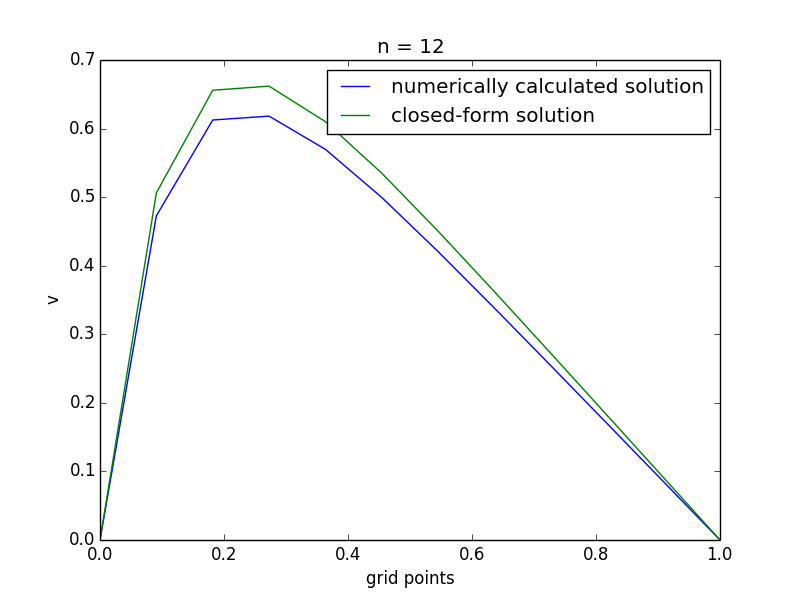
\includegraphics[width=0.7\textwidth]{blabla_12.png}
        \caption{Numerical solution against the analytical one for \(n = 12\) grid points} 
    \end{figure}

\begin{figure}[H]
            \centering % center the image horizontally
            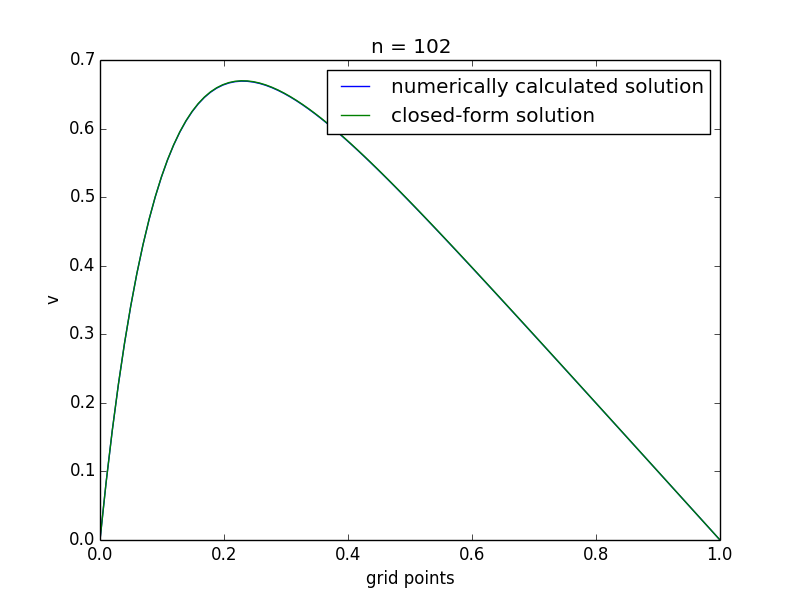
\includegraphics[width=0.7\textwidth]{blabla_102.png}
            \caption{Numerical solution against the analytical one for \(n = 102\) grid points} 
            \end{figure}   

 \begin{figure}[H]
            \centering % center the image horizontally
            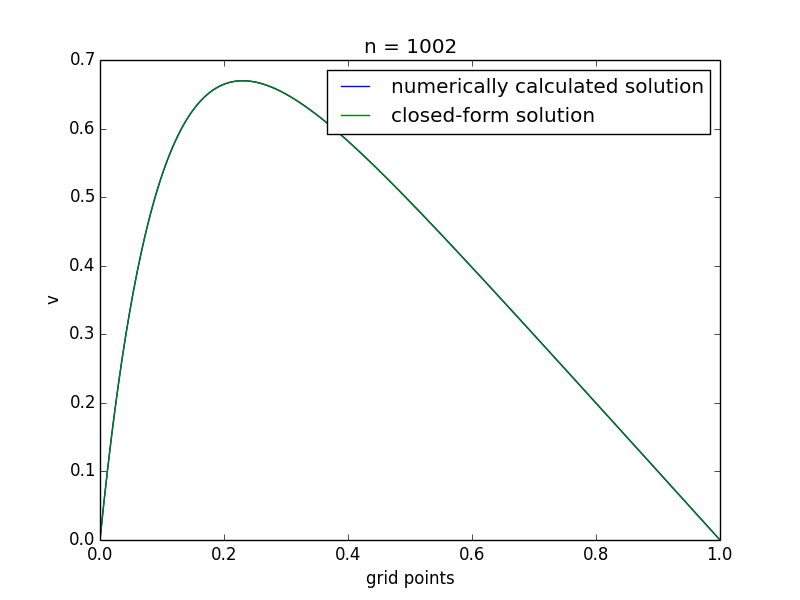
\includegraphics[width=0.7\textwidth]{blabla_1002.png}
            \caption{Numerical solution against the analytical one for \(n = 1002\) grid points} 
            \end{figure}  

\subsection{Relative error}

The relative error without taking \(log_{10}\)
is given in the table below. 

\begin{tabular}{c | l  }
    \label{pos_mikro}
    \(n\) & relative error \\ \hline
    \(10\) & \(0.066153\) \\ 
    \(100\) & \(0.000816513\)\\
    \(10^4\) & \(8.33134 e-8\)\\
    \(10^5\) & \(1.43558 e-9\)\\
    \(10^6\) & \(8.40478 e-7\)\\
    \(10^8\) & \(0.0339039\) \\\\
    \end{tabular} 

To get a nice plot of the relative error, \(log_{10}\) is taken on both axis.

\begin{figure}[H]
    \label{fig_error}
    \centering % center the image horizontally
    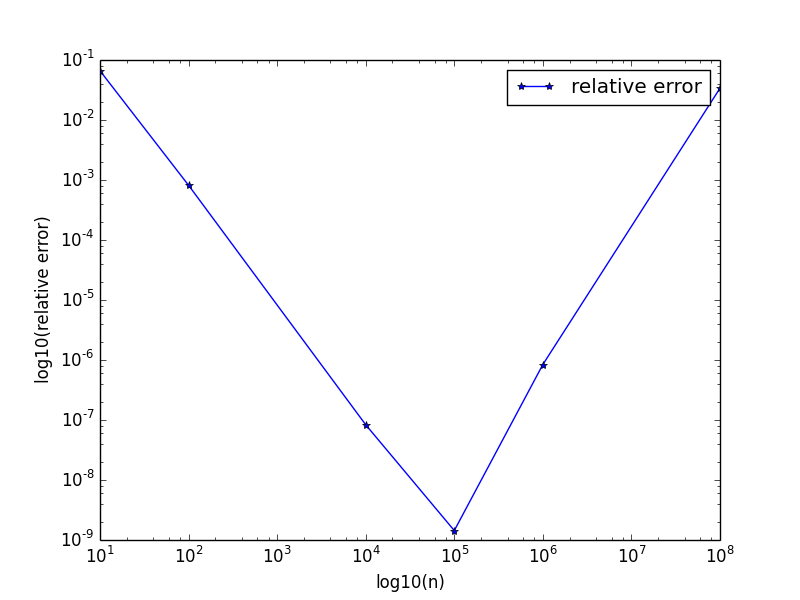
\includegraphics[width=0.7\textwidth]{relative_error.png}
    \caption{\(log_{10}\) of the relative error plottet against \(log_{10}(n)\) } 
    \end{figure} 

\subsection{CPU time}

The CPU time for the different functions containing the three
algorithms is shown in the table below.\\\\ 

\begin{tabular}{c | l | l | l }
    & \multicolumn{3}{|c|}{CPU time for three different methods [s]} \\ 
    \hline
    \(n\) & general method & specialized method & LU-decomposition\\
    \hline
    \(10\) & \(5e-6\) & \(4e-6\) & \(8.8e-5\) \\
    \(100\) & \(1.4e-5\) & \(1.2e-5\) & \(0.000883\) \\
    \(1000\) & \(8.4e-5\) & \(7.3e-5\) & \(0.060\) \\
    \(10^6\) & \(0.077\) & \(0.058\) & error \\
    \(10^7\) & \(0.74\) & \(0.56\) & error\\
    \hline
    \end{tabular} 

\section{Concluding remarks}

Looking at the three plots in section ~\ref{subsec:resplot}, it is obvious
that the numerical solution gets more accurate with a higher number of time steps. 
When looking at the plots for \(n = 102\) and \(n = 1002\) there is not much visible 
difference, but looking at table ~\ref{pos_mikro} we see that the relative error 
is much lower for \(n = 1002\). 

From figure ~\reg{fig:error} we see that the assumption that the relative error
would get higher when n became too high is correct. It also shows that you will
get the lowest relative error around \(n = 10^5\). 

The table showing CPU time shows a little difference between the general and the
special solution. The general solution is running with approximately \(8n\) floating point 
operations, and the special is running with approximately \(6n\). 
The LU-decomposition is running with \(\mathcal{O}(n^3)\) floating point operations, and we can see
that it is significantly slower that the two others. 
This is because the LU-decomposition does not take into account that we are working
in a tridiagonal matrix, and therefore works on the whole matrix instead of only 
three vectors, or constants.
For a whole matrix with different numbers for each element, the specialized algorithm 
would be useless.
If the general solution from this task was supposed to take a whole matrix and do
the same row reduction, it would use \(\mathcal{O}(n^4)\) floating point operation,
and therefore be less effective than the LU-decomposition. 
The only reason the generalized and the special algorithms are faster, is because
we are looking at a tridiagonal matrix. 

The fact that the LU-decomposition takes a whole \(n x n\)matrix instead of vectors is also the
reason why we can't run this method for \(n = 10^6\).

\section{references} 
Hjort-Jensen,M., 2016. Project 1, accessible at course github repository. 5 pages. 

Hjort-Jensen,M., 2015. Lecture notes, accessible at course github repository. 563 pages. 
\end{document}                          
